\section{Modifying the controller with $\tilde{\omega}$}

Let's consider another modified version of the control law

$$\boldsymbol{\tau} = -\mathbf{K}_d \boldsymbol{\tilde \omega} - k_p  \boldsymbol{\tilde \epsilon} $$

Where $\boldsymbol{\tilde \epsilon}$ is defined as before and $\boldsymbol{\tilde \omega} = \boldsymbol{\omega - \omega_d}. $ $\boldsymbol{\omega}_d$ is given by the reference signals from the previous problem.\\


To calculate $\boldsymbol{\omega_d}$, we will be using equation (2.26) and (2.27) in Fossen\cite{bok}:
$$ \boldsymbol{\omega_d} = \mathbf{T}_{\Theta_d}^{-1}(\Theta_d) \dot \Theta_d $$


$$ \boldsymbol{\omega_d} = \m{\dot \phi \\ 0 \\ 0} + \mathbf{R_{x, \phi}^\top} \m{0 \\ \dot \theta \\ 0} + \mathbf{R_{x, \phi}^\top} \mathbf{R_{y, \theta}^\top} \m{0 \\ 0 \\ \dot \psi} $$
$$ = \m{\cos{(0.1t)} \\ 0 \\ 0} + \m{1 && 0 && 0 \\ 0 && c\phi && s\phi \\ 0 && -s\phi && c\phi} \m{c\theta && 0 && -s\theta \\ 0 && 1 && 0 \\ s\theta && 0 && c\theta} \m{0 \\ 0 \\ -0.75 \sin{0.05t}}$$
$$ = \m{\cos{0.01t} - \sin\theta \cdot 0.75 \sin{0.05t} \\ \cos \theta \sin\phi \cdot 0.75 \sin{0.05t} \\ \cos \theta \cos \phi  \cdot 0.75 \sin{0.05t} } $$
Now we will simulate the system with this second modified control law using the same parameters, initial conditions and reference signals as in section 5.

See figure \ref{fig:eulang3}, \ref{fig:eulang_tilde3} and \ref{fig:tau3} for the plots of the Euler angles (both actual and desired) and angular velocities ($\phi, \phi_d, \theta, \theta_d, \psi, \psi_d, \boldsymbol{\omega}$), the Euler angles error ($\tilde \phi, \tilde \theta, \tilde \psi$) and the control inputs ($\boldsymbol{\tau}$).

After introducing desired angular velocities $\boldsymbol{\omega_d}$ that match the desired angles, the system behaves according to our expectations. The angles are able to follow their desired state, even the sinusoidal ones, because the forces controlling the angles and the angular velocity are working together.


\begin{figure}[h!]
    \centering
    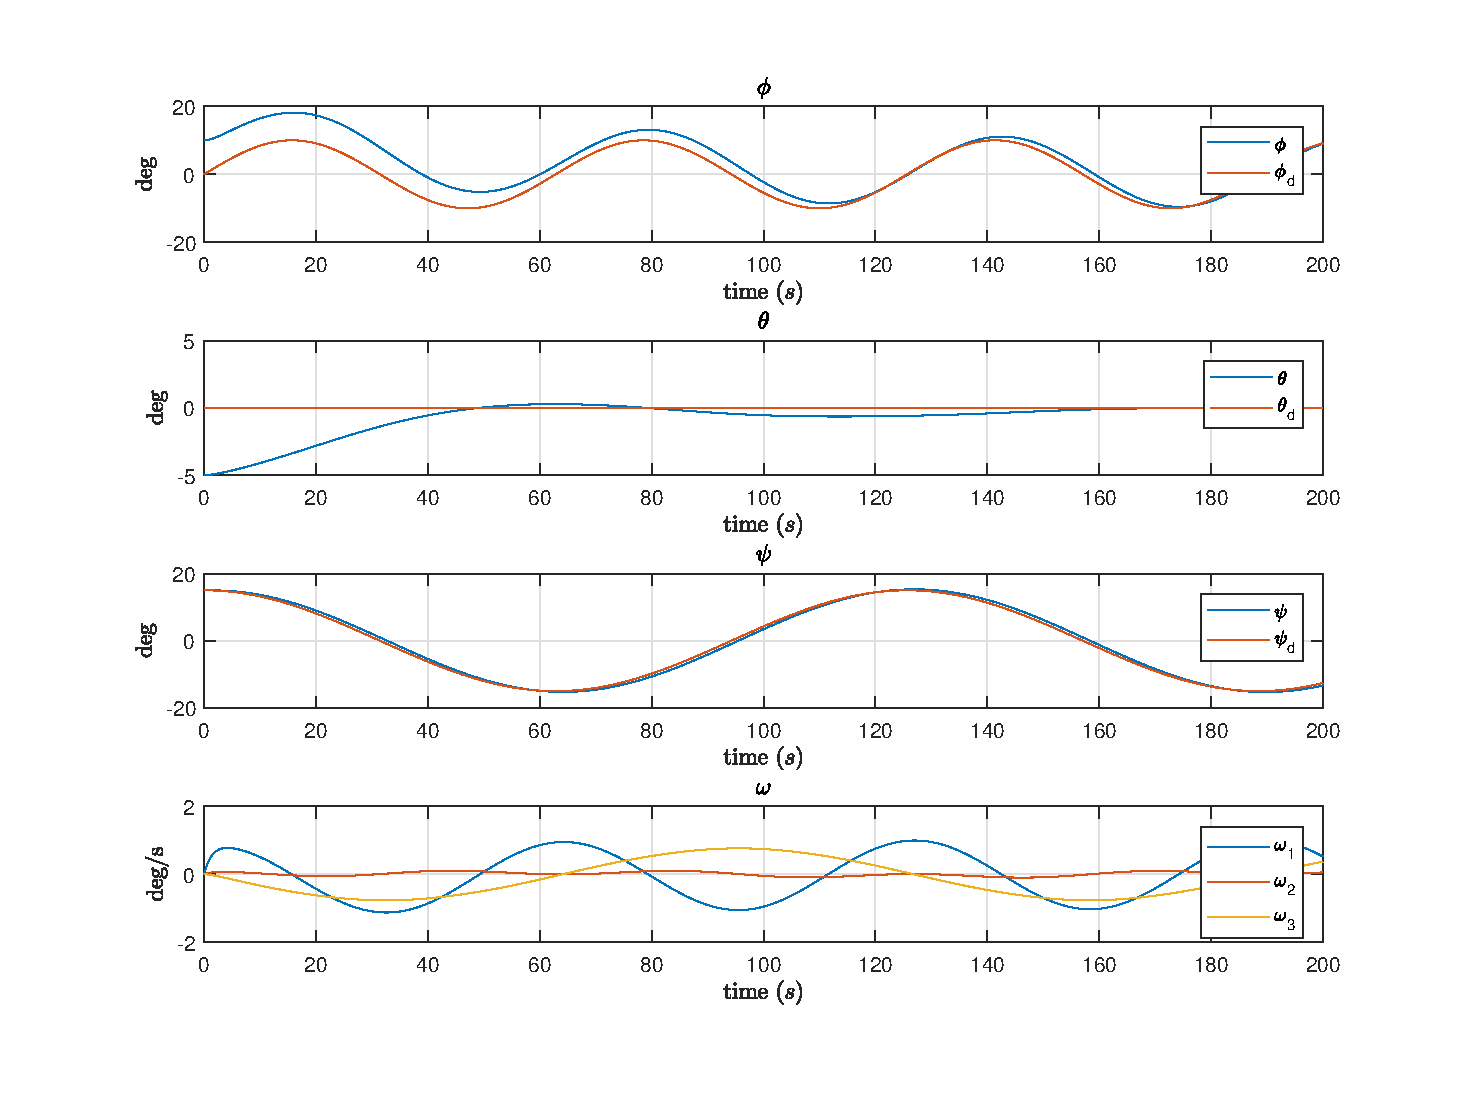
\includegraphics[scale=0.6]{eulang3.eps}
    \caption{Simulated Euler angles, desired Euler angles and angular velocity}
    \label{fig:eulang3}
\end{figure}

\begin{figure}[h!]
    \centering
  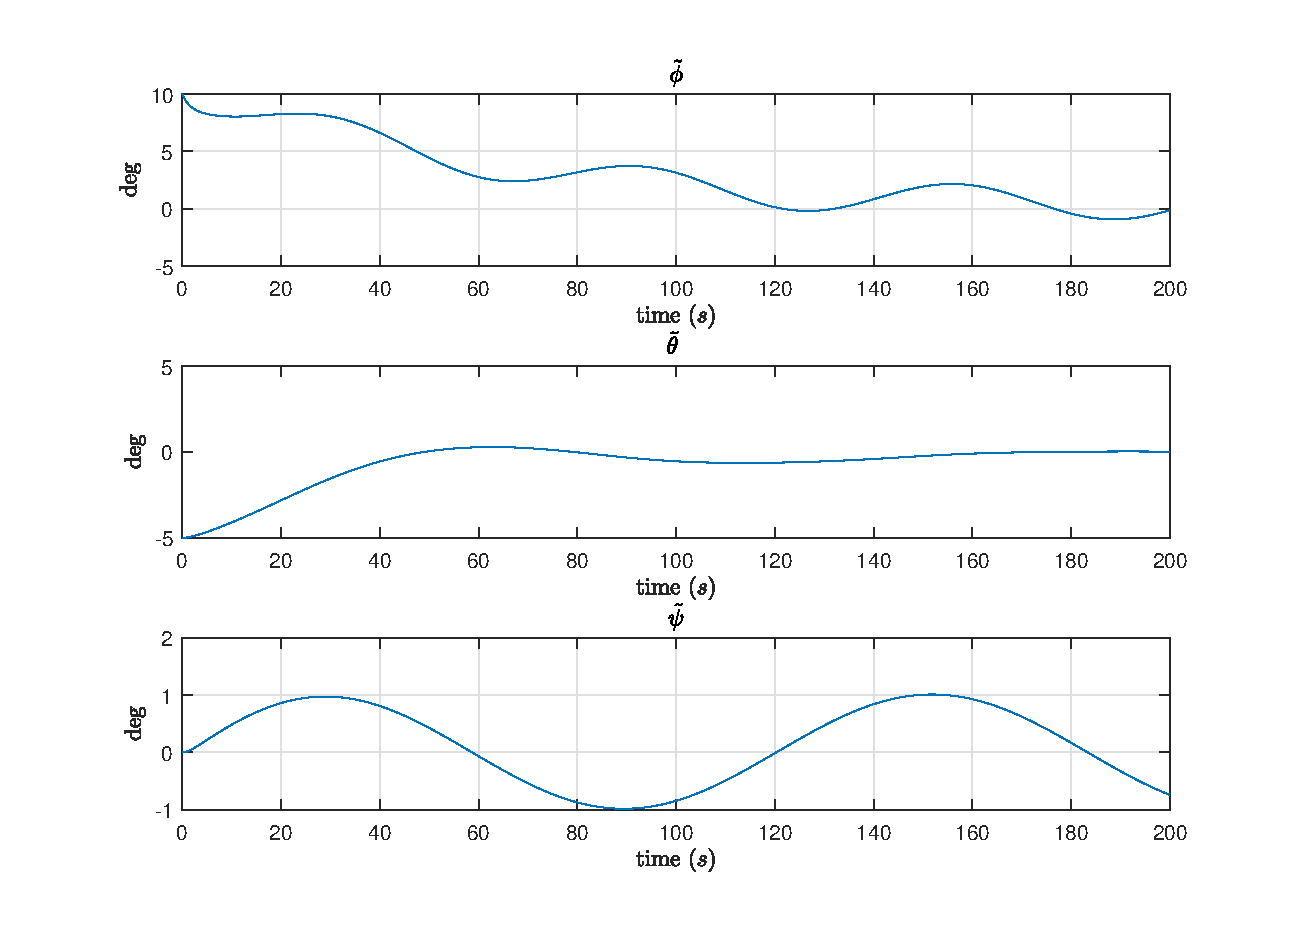
\includegraphics[scale=0.7]{eulang_tilde3.eps}
  \caption{Simulated Euler angles tracking error}
  \label{fig:eulang_tilde3}
\end{figure}


\begin{figure}[h!]
    \centering
    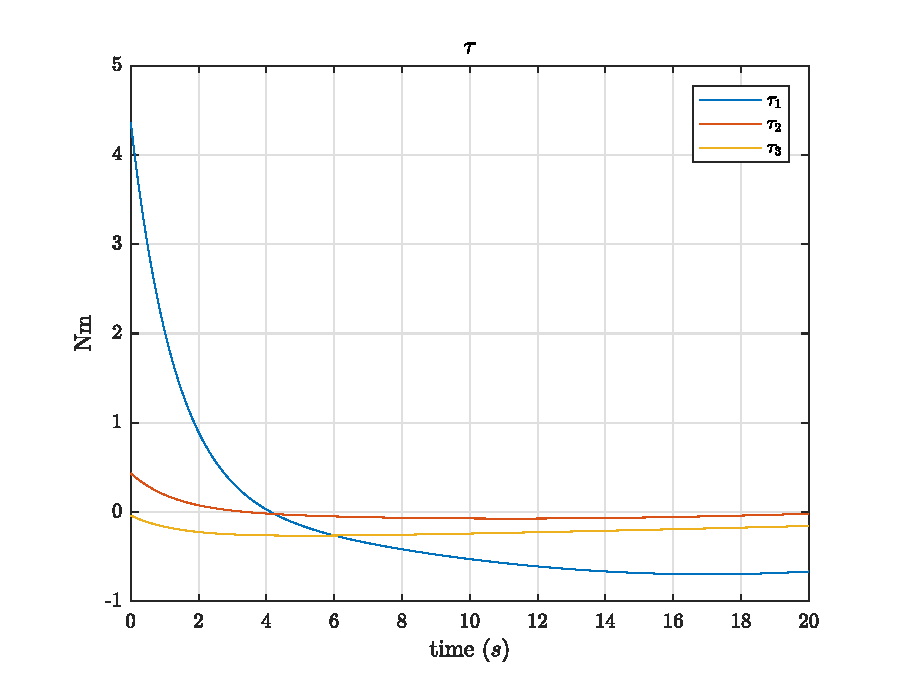
\includegraphics[scale=0.7]{tau3.eps}
    \caption{Simulated control input $\tau$}
    \label{fig:tau3}
\end{figure}


